% Options for packages loaded elsewhere
\PassOptionsToPackage{unicode}{hyperref}
\PassOptionsToPackage{hyphens}{url}
\documentclass[
]{article}
\usepackage{xcolor}
\usepackage[margin=1in]{geometry}
\usepackage{amsmath,amssymb}
\setcounter{secnumdepth}{-\maxdimen} % remove section numbering
\usepackage{iftex}
\ifPDFTeX
  \usepackage[T1]{fontenc}
  \usepackage[utf8]{inputenc}
  \usepackage{textcomp} % provide euro and other symbols
\else % if luatex or xetex
  \usepackage{unicode-math} % this also loads fontspec
  \defaultfontfeatures{Scale=MatchLowercase}
  \defaultfontfeatures[\rmfamily]{Ligatures=TeX,Scale=1}
\fi
\usepackage{lmodern}
\ifPDFTeX\else
  % xetex/luatex font selection
\fi
% Use upquote if available, for straight quotes in verbatim environments
\IfFileExists{upquote.sty}{\usepackage{upquote}}{}
\IfFileExists{microtype.sty}{% use microtype if available
  \usepackage[]{microtype}
  \UseMicrotypeSet[protrusion]{basicmath} % disable protrusion for tt fonts
}{}
\makeatletter
\@ifundefined{KOMAClassName}{% if non-KOMA class
  \IfFileExists{parskip.sty}{%
    \usepackage{parskip}
  }{% else
    \setlength{\parindent}{0pt}
    \setlength{\parskip}{6pt plus 2pt minus 1pt}}
}{% if KOMA class
  \KOMAoptions{parskip=half}}
\makeatother
\usepackage{longtable,booktabs,array}
\usepackage{calc} % for calculating minipage widths
% Correct order of tables after \paragraph or \subparagraph
\usepackage{etoolbox}
\makeatletter
\patchcmd\longtable{\par}{\if@noskipsec\mbox{}\fi\par}{}{}
\makeatother
\usepackage{graphicx}
\makeatletter
\newsavebox\pandoc@box
\newcommand*\pandocbounded[1]{% scales image to fit in text height/width
  \sbox\pandoc@box{#1}%
  \Gscale@div\@tempa{\textheight}{\dimexpr\ht\pandoc@box+\dp\pandoc@box\relax}%
  \Gscale@div\@tempb{\linewidth}{\wd\pandoc@box}%
  \ifdim\@tempb\p@<\@tempa\p@\let\@tempa\@tempb\fi% select the smaller of both
  \ifdim\@tempa\p@<\p@\scalebox{\@tempa}{\usebox\pandoc@box}%
  \else\usebox{\pandoc@box}%
  \fi%
}
% Set default figure placement to htbp
\def\fps@figure{htbp}
\makeatother
\setlength{\emergencystretch}{3em} % prevent overfull lines
\providecommand{\tightlist}{%
  \setlength{\itemsep}{0pt}\setlength{\parskip}{0pt}}
\usepackage{hyperref}
\IfFileExists{xurl.sty}{\usepackage{xurl}}{} % add URL line breaks if available
\urlstyle{same}
\hypersetup{
  hidelinks,
  pdfcreator={LaTeX via pandoc}}

\author{}
\date{}

\begin{document}
\setlength{\parskip}{3pt plus 1pt minus 1pt}

\section{When Shared Slice Context Hides Paired Reconstruction Error: A
Two-Source Audit of Through-Plane MRI
Interpolation}\label{when-shared-slice-context-hides-paired-reconstruction-error-a-two-source-audit-of-through-plane-mri-interpolation}

\textbf{Internal scientific draft, 2026-10-01. Not a submission
package.} This version uses only the publicly licensed IXI training
source, MSValid and TCIA ReMIND patient sources for its reported
estimates and
\href{figures/PUBLIC_TWO_SOURCE_FIGURE_NOTE_2026-10-01.md}{quantitative
figure}. It excludes the older fastMRI/NingXia figures and architecture
matrix. The IXI-weight MSValid same-patient result was selected after an
earlier weight-pair result; ReMIND was frozen later, before its image
pixels were decoded. Common-scale/reverse, native-linear-partner and
matched-geometry synthetic-noise controls were designed after seeing the
corresponding main results. Original publication permissions, venue
format, reproducibility supplement and author approval remain separate
gates.

\subsection{Abstract}\label{abstract}

Agreement between two MRI slice interpolators need not reveal their
common error when both reuse the same observed slices. We quantify this
dependence with a fixed-reference, same-target audit: a frozen HAT
prediction is paired with a frozen SwinIR prediction made either from
shared or disjoint published-slice contexts. We retrospectively evaluate
the fraction of paired error visible in output disagreement, using an
IXI-T2-trained model pair and acquired-only foreground support. In a
result-after-designed, same-patient follow-up on 84 MSValid RRMS brain
T2 examinations (479 target planes), the patient-weighted
disjoint-minus-shared difference was 24.19 percentage points (95\%
patient-bootstrap interval 23.71--24.67). A later protocol-frozen test
on a different TCIA ReMIND preoperative brain-tumor source scored 62/63
patients and 248 targets, with a 26.40-point difference (95\% stratified
patient-bootstrap interval 25.69--27.17); both ReMIND 2D sequence groups
had positive point estimates. Post-result common-anchor-normalization
controls retained 24.04 and 26.32 points in MSValid and ReMIND,
respectively; reversing the fixed-reference phase retained 24.07 and
26.30 points. Replacing SwinIR with native linear interpolation still
yielded 20.54 and 22.94 points, so the direction is not specific to
learned cross-architecture pairing. In a post-result MSValid synthetic
control with identical anatomy and geometry, independent versus shared
simulated noise changed the endpoint by -0.00034 and +0.00253 points at
1\% and 5\% noise, respectively. These observations document
context-dependence of disagreement but do not isolate original
acquisition identity, certify individual reconstruction accuracy, or
test recovery of independently acquired thin slices; published ReMIND
DICOMs carry an MPR image-type flag.

\subsection{1. Introduction}\label{introduction}

Comparing two reconstruction outputs is a tempting way to assess
reliability without a ground-truth target. Yet two models may agree
because they process the same evidence and inherit aligned errors. This
possibility is established in ensemble theory and MRI error work
{[}1--3{]}. Its practical size under a controlled change of observed
slice context is less clear for through-plane interpolation.

We study a deliberately limited question. For one frozen
cross-architecture pair and one withheld published target plane, does
the fraction of paired error visible in model disagreement change when
only the companion model switches to a disjoint set of published context
slices? The fixed reference and target prevent a change of either from
explaining the contrast. The intervention still changes the companion's
complete neighboring images, signed geometry and potentially
preprocessing, so the resulting estimate is a \emph{context contrast},
not an identity-only causal effect.

Our contribution is an auditable fixed-pair protocol and its
source-specific evaluation on two public patient collections with
distinct disease contexts. The analysis keeps retrospective error
observability separate from deployable confidence: the former requires
the withheld target for evaluation. This distinction matters because
supervised MRI error estimators and calibrated uncertainty intervals
already address different downstream questions {[}1,4{]}; no such
performance is claimed here.

\subsection{2. Prior Work and Claim
Boundary}\label{prior-work-and-claim-boundary}

Hu et al.~{[}1{]} explicitly show that MRI prediction variability can
miss systematic error and train an error-prediction model. Classical
ambiguity and negative-correlation analyses {[}2,3{]} likewise establish
that correlated errors affect ensemble behavior. Our distinction is the
paired, fixed-reference intervention on published physical slice
contexts under an explicit information contract, with full patient-level
accounting and a second patient source. We do not claim discovery of
common error or a new energy identity.

HAT and SwinIR {[}5,6{]} are image-restoration architectures used here
through frozen local 2.5D MRI training wrappers, not official MRI
checkpoints. Through-plane interpolation and complementary-slice
acquisition predate this study {[}7{]}. Recent supervised pixelwise MRI
intervals {[}4{]} and range/null ambiguity decomposition {[}8{]} cover
uncertainty and identifiability concepts that should not be relabeled as
our innovation. They address different forward operators, training
targets or guarantees; our endpoint remains retrospective paired-error
visibility for the tested slice contexts.

Two further MRI precedents narrow the language. A measured-subspace audit
of diffusion posterior samples tests whether reconstructions conditioned
on one fixed multi-coil k-space measurement disagree on already acquired
coefficients, then applies a consistency lock {[}12{]}.
Input-perturbation/local-Lipschitz work relates output response to MRI
reconstruction error and proposes an action threshold {[}13{]}. Neither
measures the present same-target published-slice context contrast, but
they preclude a broad claim to originate black-box measurement auditing
or sensitivity-based reliability scoring. Our analysis changes a
companion's published context and requires target truth; it supplies
neither a k-space consistency guarantee nor a deployable threshold.

\subsection{3. Data and Frozen
Inference}\label{data-and-frozen-inference}

\textbf{Training source and models.} Both checkpoints are local
HAT/SwinIR 2.5D implementations trained on public IXI T2 {[}9{]} and
fixed before these analyses. The stored checkpoint SHA-256 values and
inference script hashes appear in the
\href{MSVALID_IXI_WEIGHTS_SECONDARY_RESULT_2026-10-01.md}{MSValid
result} and
\href{REMIND_NATIVE_T2_CONFIRMATION_PROTOCOL_2026-10-01.md}{ReMIND
protocol}. Inference uses CPU float32 and two PyTorch threads; no new
training is included in this paper.

\textbf{MSValid.} The public Zenodo collection {[}10{]} contributes the
first available T2 volume for each of 84 geometry-qualified RRMS
patients. There are 479 preselected residue-1/3 published target planes.
Native through-plane spacing is 3--6 mm. This analysis reuses patients
already evaluated with another weight pair; the IXI weight-pair
comparison was fixed only after that earlier result had been inspected.
It is therefore a same-patient secondary result, not an independent
source confirmation of the original discovery.

\textbf{ReMIND.} Official TCIA/NBIA downloads {[}11{]} supply all 63
available preoperative \texttt{2D\_AX\_T2} (36 patients) and
\texttt{2D\_AX\_T2\_BLADE} (27 patients) series in the frozen inventory,
without patient overlap between these two protocol groups. Header-only
checks excluded one ordinary-T2 series with 21 layers under the
predeclared 24-layer threshold, leaving 35 ordinary and 27 BLADE
patients. Each contributed two targets in each residue class, 248
targets overall. The median released z spacing is about 5.0 mm in
ordinary T2 and 2.5 mm in BLADE. DICOM \texttt{ImageType} includes
\texttt{MPR} across both groups; neither series label nor layer geometry
proves that published slices are independently acquired raw planes. The
protocol was written after the MSValid result but before any ReMIND
target pixels were decoded.

\textbf{Target and context contract.} Physical layer locations, not
filenames or DICOM InstanceNumber, determine ReMIND z order. With
zero-based ordered planes, phase 0 contains \texttt{0,4,8,...} and phase
2 contains \texttt{2,6,10,...}. Targets have residue 1 or 3 and
sufficient real planes on both sides. HAT phase 0 supplies fixed
prediction \texttt{a}. SwinIR phase 0 supplies shared partner
\texttt{b\_s}; SwinIR phase 2 supplies disjoint partner \texttt{b\_d},
predicting the same withheld target \texttt{y}. The original models
normalize each input phase from all its observed anchors, resize to 256
x 256 and use a four-channel left/right/linear-coarse/relative-position
condition; the output residual is returned to native in-plane size and
intensity range. ReMIND DICOM rescale slope/intercept is applied per
plane. Inputs never use the target pixel intensities. A post-result
negative control replaces each SwinIR partner with native-intensity
linear interpolation of its two real bracketing planes at the same
quarter/three-quarter index offset; the HAT reference, target, support
and patient aggregation stay fixed.

\textbf{Evaluation support.} The foreground support is the union of
pixels exceeding 1\% of each nearest phase-0 anchor's maximum absolute
intensity. It is determined from observed anchors alone and held fixed
between the two companion conditions. This support is not a lesion mask.
The reference output \texttt{a}, target \texttt{y} and support are
exactly shared across the paired comparison.

\subsection{4. Estimand and Statistical
Unit}\label{estimand-and-statistical-unit}

For errors \texttt{e\_a=a-y} and \texttt{e\_b=b-y} on the fixed support,
define

\[
T=\frac{\operatorname{MSE}(a,y)+\operatorname{MSE}(b,y)}{2},\qquad
O=\frac{\operatorname{mean}[(a-b)^2]}{4T}.
\]

\texttt{O} is the fraction of paired error energy visible in
disagreement, with retrospective access to \texttt{y} only for
evaluation. The principal source-specific contrast is
\texttt{Delta\ O\ =\ O(a,b\_d,y)-O(a,b\_s,y)}. For each patient, targets
are first averaged within residue 1/3, then the two residues are equally
weighted; patients are the independent units. MSValid reports its frozen
5,000-draw patient bootstrap interval. ReMIND uses its frozen 5,000-draw
bootstrap stratified by the two 2D protocol groups, weighting strata by
completed patient counts. We report group estimates without treating
targets or the two protocol groups as additional independent
confirmations.

An exact algebraic identity expresses \texttt{O} through paired-error
cosine and the two MSE terms. This identity is a diagnostic, not a new
theorem or independent experiment. The output difference alone does not
measure total error and cannot be used as a calibrated patient-level
error score from the present data.

\subsection{5. Results}\label{results}

\begin{longtable}[]{@{}
  >{\raggedright\arraybackslash}p{(\linewidth - 4\tabcolsep) * \real{0.2727}}
  >{\raggedleft\arraybackslash}p{(\linewidth - 4\tabcolsep) * \real{0.3636}}
  >{\raggedleft\arraybackslash}p{(\linewidth - 4\tabcolsep) * \real{0.3636}}@{}}
\toprule\noalign{}
\begin{minipage}[b]{\linewidth}\raggedright
Patient-level endpoint
\end{minipage} & \begin{minipage}[b]{\linewidth}\raggedleft
MSValid, IXI-weight follow-up
\end{minipage} & \begin{minipage}[b]{\linewidth}\raggedleft
ReMIND, later frozen source test
\end{minipage} \\
\midrule\noalign{}
\endhead
\bottomrule\noalign{}
\endlastfoot
Completed patients / fixed targets & 84/84; 479 & 62/63; 248 \\
Shared \texttt{O} & 1.0420\% & 1.1093\% \\
Disjoint \texttt{O} & 25.2276\% & 27.5092\% \\
\texttt{Delta\ O} & +24.1856 percentage points & +26.3999 percentage
points \\
95\% patient-bootstrap interval & +23.7150 to +24.6726 & +25.6945 to
+27.1686 \\
Positive patient differences & 84/84 & 62/62 \\
SwinIR shared/disjoint MAE, within-scan units & 130.33 / 129.46 & 132.13
/ 131.71 \\
\end{longtable}

The patient-level figure plots every paired patient result and labels
the evidence order. Numerical differences between collections cannot be
interpreted as disease effects: acquisition, published processing,
target geometry and analysis chronology all differ.

\begin{figure}
\centering
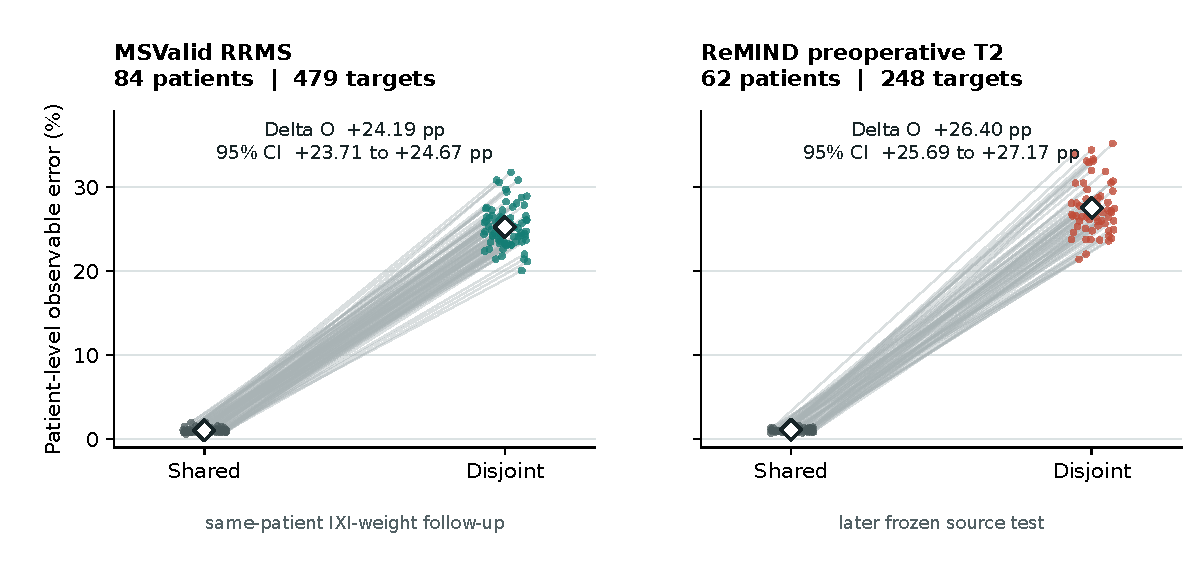
\includegraphics[width=0.88\linewidth,height=\textheight,keepaspectratio,alt={Patient-level observable paired-error percentages for the fixed IXI-trained HAT/SwinIR pair across MSValid and ReMIND. Gray segments connect the same patient's shared and disjoint contexts; white diamonds mark patient means. The two tests have different design histories and are not a controlled cross-disease comparison.}]{figures/public_two_source_observability.pdf}
\caption{Patient-level observable paired-error percentages for the fixed
IXI-trained HAT/SwinIR pair across MSValid and ReMIND. Gray segments
connect the same patient's shared and disjoint contexts; white diamonds
mark patient means. The two tests have different design histories and
are not a controlled cross-disease comparison.}
\end{figure}

ReMIND's ordinary-T2 group had a +26.5156-point mean (35/35 positive);
BLADE had +26.2500 points (27/27 positive). Both groups met their
prespecified count and direction thresholds; the pooled interval lower
bound exceeded zero. The only failure was the documented pre-pixel short
series. Result-after common min/max controls used the union of real
anchors for both phase normalizations and yielded +24.0358 points on
\href{MSVALID_IXI_WEIGHT_POSTRESULT_CONTROLS_RESULT_2026-10-01.md}{MSValid}
and +26.3236 on
\href{REMIND_POSTRESULT_CONTROLS_RESULT_2026-10-01.md}{ReMIND}. Fixing
HAT phase 2 and using a phase-2 acquired-only support yielded +24.0681
and +26.3049 points, respectively. All 84 MSValid and 62 ReMIND patient
differences remained positive in both exploratory directions. These
checks rule out independent min/max and one chosen reference phase as
sole explanations, but not neighboring image content or geometry.

The
\href{PUBLIC_LINEAR_PARTNER_CONTROL_RESULT_2026-10-01.md}{post-result
native-linear partner control} reused every original target, fixed HAT
prediction and support. Its shared/disjoint \texttt{O} was
5.8641\%/26.4085\% on MSValid and 5.6629\%/28.6015\% on ReMIND;
patient-weighted \texttt{Delta\ O} remained +20.5445 points (95\%
patient-bootstrap interval +20.1283 to +20.9729; 84/84 positive) and
+22.9386 points (95\% stratified patient-bootstrap interval +22.3772 to
+23.5257; 62/62 positive). Both ReMIND 2D groups were positive. This
directly limits a learned-pair-specific reading of the main result.
Because the linear and SwinIR partners have different errors and
\texttt{O} uses each partner's MSE in its denominator, subtracting their
contrasts does not identify a neural-network contribution.

The
\href{MSVALID_MATCHED_GEOMETRY_NOISE_CONTROL_RESULT_2026-10-01.md}{post-result
matched-geometry synthetic-noise control} kept both networks on the same
phase-0 anatomical planes, locations and clean-anchor normalization
range, changing only whether SwinIR shared HAT's generated
magnitude-noise realization. On all 84 MSValid patients and 479 targets
per level, independent-minus-shared \texttt{O} was -0.000339 percentage
points at 1\% noise (95\% patient-bootstrap interval -0.001348 to
+0.000604; 41/84 positive) and +0.002529 points at 5\% noise (+0.000276
to +0.004900; 46/84 positive). Both magnitudes are small compared with
the original +24.1856-point phase contrast. The 5\% interval excludes
zero, but this is an arbitrary synthetic perturbation on already
published magnitude planes, not a repeated acquisition; its result
cannot apportion the original contrast among noise identity, anatomy and
geometry.

In a
\href{FIXED_DENOMINATOR_TWO_SOURCE_RESULT_2026-10-01.md}{post-result
fixed-denominator sensitivity}, both conditions for each target used the
shared-condition paired MSE in the denominator. Patient-weighted
disjoint-minus-shared disagreement remained +24.2152 points on MSValid
(95\% patient-bootstrap interval +23.6886 to +24.7320) and +26.4918
points on ReMIND (+25.7382 to +27.2917). All 479 and 248 original
targets, respectively, increased in raw squared output disagreement.
This excludes a changing paired-MSE denominator as the sole explanation,
but recomputes the same predictions and cannot distinguish anatomy,
geometry or acquisition identity.

In a result-after
\href{REMIND_ERROR_ALIGNMENT_DECOMPOSITION_RESULT_2026-10-01.md}{algebraic
decomposition}, companion MSE imbalance contributed +0.0779 points and
the error-alignment component +26.3220 points to the original ReMIND
\texttt{Delta\ O}; the terms close the observed effect by identity, so
this is explanation of the measured endpoint rather than new evidence.

\subsection{6. Discussion and
Limitations}\label{discussion-and-limitations}

Across the tested pair, a small shared-context disagreement coexists
with substantial paired error, while a disjoint published-slice context
exposes more of that error. The fixed target and HAT output make this
more specific than an unpaired comparison of two reconstruction methods.
A simple linear partner preserves much of the contrast; shared-input
dependence is therefore not unique to two learned architectures. Under
matched published anatomy and geometry, changing only simulated noise
identity did not reproduce the large phase contrast. This does not show
that actual acquisition identity is irrelevant: the simulation uses
arbitrary noise levels, a magnitude-noise approximation and clean-anchor
normalization, and cannot mimic motion or the acquisition/reconstruction
chain. The original intervention still changes complete neighboring
planes and signed relative positions. The per-phase input range may also
change; common-scale sensitivity controls only that range difference and
leaks two extrema from the other phase into the shared condition.
ReMIND's MPR DICOM flag further prevents an inference about independent
original acquisition events. No actual thick-to-thin acquisition, lesion
preservation, diagnostic decision or clinical outcome was tested.

Mean error visibility is distinct from identifying a higher-error
target. In a
\href{TWO_SOURCE_TARGET_ERROR_RANKING_RESULT_2026-10-01.md}{post-result
within-patient, within-residue ranking check}, HAT/SwinIR
output-disagreement concordance increased from 0.661 to 0.802 on MSValid
but only from 0.613 to 0.677 on ReMIND; the latter's paired patient
interval for the improvement crossed zero. Disjoint SwinIR exceeded a
disjoint native-linear score in both sources, but the phase-2 images
required by both disjoint scores are unavailable under the intended
phase-0-only x4 input. These findings do not establish a deployable or
calibrated error score.

The public-source route deliberately drops the older fastMRI/NingXia
matrix. It therefore does not claim broad architecture replication, a
new interpolator or calibrated case-level risk prediction. The MSValid
IXI-weight result reused patients after an earlier result influenced
model-pair selection, and ReMIND was chosen with that history known.
Patient bootstrap intervals describe sampling within these fixed
cohorts, not research-selection uncertainty. Anonymous identifiers
cannot prove absolute cross-collection patient non-overlap. Raw
intensity MAE is meaningful only within paired scans and does not
compare disease groups in physical units.

This audit's practical message is limited but direct: agreement between
frozen interpolators that reuse the same published slices should not be
treated as independent evidence of correctness, whether the partner is
another network or simple interpolation. A future study that seeks a
stronger acquisition-identity claim needs sequence provenance
establishing which planes are independently acquired, matched
geometry/content controls, and a prospectively isolated target. A
deployable detector additionally requires an acquired-only score and
external ranking/calibration tests against supervised error methods
{[}1,4{]}.

\subsection{References to verify in venue
style}\label{references-to-verify-in-venue-style}

\begingroup\fontsize{9}{10.5}\selectfont
\begin{enumerate}
\def\labelenumi{\arabic{enumi}.}
\tightlist
\item
  Hu et al.~\emph{Learning to Predict Error for MRI Reconstruction.}
  MICCAI 2021. DOI 10.1007/978-3-030-87199-4\_57.
\item
  Krogh and Vedelsby. \emph{Neural Network Ensembles, Cross Validation,
  and Active Learning.} NeurIPS 1994.
\item
  Liu and Yao. \emph{Ensemble learning via negative correlation.} Neural
  Networks 1999. DOI 10.1016/S0893-6080(99)00073-8.
\item
  Giannakopoulos et al.~\emph{Pixel-Wise Uncertainty Quantification of
  Accelerated MRI Reconstruction.} Magnetic Resonance in Medicine 2026.
  DOI \texttt{10.1002/mrm.70526}.
\item
  Chen et al.~\emph{Activating More Pixels in Image Super-Resolution
  Transformer.} CVPR 2023.
\item
  Liang et al.~\emph{SwinIR: Image Restoration Using Swin Transformer.}
  ICCV Workshops 2021.
\item
  Greenspan et
  al.~\href{https://doi.org/10.1016/S0730-725X(02)00511-8}{\emph{MRI
  inter-slice reconstruction using super-resolution.}} Magnetic
  Resonance Imaging 20(5):437--446, 2002.
\item
  Guo et al.~\emph{Separating Intrinsic Ambiguity from Estimation
  Uncertainty in Deep Generative Models for Linear Inverse Problems.}
  arXiv:2605.15050v1, 2026.
\item
  Imperial College Biomedical Image Analysis Group. \emph{IXI Dataset.}
  \href{https://brain-development.org/ixi-dataset/}{Official dataset
  page}, CC BY-SA 3.0.
\item
  Pappalardo et al.~\emph{MSValid Data Collection.} Zenodo 2024. DOI
  \texttt{10.5281/zenodo.10875606}, CC BY 4.0.
\item
  Juvekar, P., Dorent, R., Kögl, F., Torio, E., Barr, C., Rigolo, L.,
  Galvin, C., Jowkar, N., Kazi, A., Haouchine, N., Cheema, H., Navab,
  N., Pieper, S., Wells, W. M., Bi, W. L., Golby, A., Frisken, S., \&
  Kapur, T. (2023). \emph{The Brain Resection Multimodal Imaging Database
  (ReMIND)} (Version 1) {[}dataset{]}. The Cancer Imaging Archive.
  \href{https://doi.org/10.7937/3RAG-D070}{DOI
  10.7937/3RAG-D070}.
\item
  Lee and Choi. \emph{Measured-Subspace Consistency: A Plug-and-Play
  Operator for Diffusion Posterior Sampling in Accelerated MRI
  Reconstruction.} arXiv:2606.28448v1, 2026.
\item
  Bhutto et al. \emph{Uncertainty Estimation and Out-of-Distribution
  Detection for Deep Learning-Based Image Reconstruction using the Local
  Lipschitz.} arXiv:2305.07618v3, 2023.
\end{enumerate}
\endgroup

\end{document}
